\section{Motion sensors as input devices}




\section{Gestures}
A gesture can be defined as a physical movement of the hands, arms, face and body with the intent to convey information or meaning~\citep{Mitra2007}, 
Even though the use of keyboard and mouse is a prominent interaction method, there are situations in which
these devices are impractical for human-computer interaction (HCI). This is particularly the case for interaction with 3D objects~\citep{Rautaray2015}. 

To be able to convey semantically meaningful commands through the use of gestures one must rely on a gesture recognition system, 
which is responsible for capturing and interpreting gestures from the user and, if applicable, carry out the desired action. 
Often this process is seen as a sum of three fundamental phases: Detection, tracking and recognition~\citep{Rautaray2015}.



\section{Gesture Recognition Principles}
This section will describe what makes up a gesture recogntion system.

\subsection{Detection}
The first step in a typical gesture recognition system is to detect the relevant parts of the captured image and segment them from the rest. 
This segmentation is crucial because it isolates the relevant parts of the image from the background to ensure that only the relevant part is processed by the subsequent 
tracking and recognition stages~\citep{Cote2006}. 
A gesture recognition system will typically be interested in hand gestures, head- and arm movements and body poses, and thus only these factors should be observed by the system.

\subsection{Tracking}
The second step in a gesture recognition system is to track the movements of the relevant segments of the frames, e.g.~the hands. 
Tracking can be described as the frame-to-frame correspondence of the segmented hand regions and aims to understand the observed hand movements. 
This is often a difficult task as hands can move very fast and their appearance can change vastly within a few frames, 
especially when light condition is a big factor~\citep{Wang2010}. 
One additional note is that if the detection method used is fast enough to operate at image acquisition frame rate, it can also be used for tracking~\citep{Rautaray2015}.   

\subsection{Recognition}
The last step of a gesture recognition system is to detect when a gesture occurs. 
This often implies checking against a predefined set of gestures, each entailing a specific action. 
To detect static gestures (i.e postures involving no movement) a general classifier or template-matcher can be used, 
but with dynamic gestures (which involves movement) other methods, which keep the temporal aspect, such as a Hidden Markov Model (HMM), are often required~\citep{Benton1995}. 
The recognition technology often makes uses of several methods from the field of machine learning, including supervised, unsupervised and reinforced learning.

When a gesture recognition system detects a relevant segment, it is thus tracked and represented in some way in the system. For hand gesture representations, 
which is the most relevant for this thesis, there are two major categories of hand gesture representations: 3D model-based methods and appearance-based methods~\citep{Rautaray2015}.

\begin{figure}%[h!] %[H]
	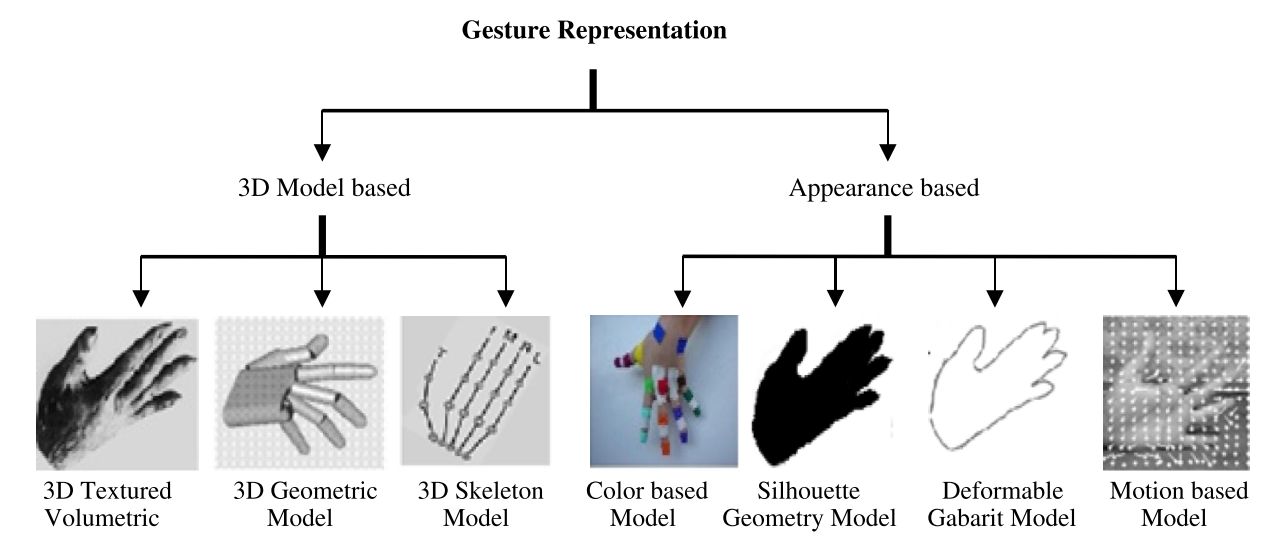
\includegraphics[width=\linewidth]{pictures/gesture_representation.png}
	\caption[Vision-based hand gesture representations]{Vision-based hand gesture representations~\citep{Bourke2007} }
	\label{fig:oculus}
\end{figure}


\section{Challenges with VR and GRT} 
Problems with using VR + e.g Leap over mouse + keyboard + display. E.g:

\subsection{The "writing issue"}
Virtual keyboards are bad. 
Regular keyboards are impractical. 
See "ideer til masteroppgaven.txt"

\subsection{Challenges in "designing" gesture schemes}
People have different preferences. Have intuitive gestures. Have gestures that is not too
fatiguing. Have gesture with high precision and recall (F-score) (high TP and TN. Low FP, FN).
Have a system that doesnt mistake one gesture for another.

\subsubsection{Fixes?}
User-gesture calibration. 

\section{Related work}